\documentclass[10pt]{beamer}

\usetheme[progressbar=frametitle]{metropolis}
\setbeamercolor{frametitle}{bg=black!85, fg=white}
\setbeamercolor{progress bar}{fg=cyan!70!blue}
\setbeamercolor{alerted text}{fg=cyan!80!blue}
\setbeamercolor{normal text}{fg=white, bg=black!88}

\usepackage{booktabs}
\usepackage{graphicx}
\usepackage{hyperref}
\usepackage{pgfplots}
\pgfplotsset{compat=1.18}

\definecolor{auditor}{HTML}{4E79A7}
\definecolor{advocate}{HTML}{59A14F}
\definecolor{skeptic}{HTML}{E15759}
\definecolor{boundary}{HTML}{F28E2B}
\definecolor{testfoc}{HTML}{B07AA1}

\title{WaRF}
\subtitle{When AI Reviewers Fight}
\author{Teymur Heydarov}
\institute{SoCraTes Austria 2026}
\date{25 September 2026}

\begin{document}

\maketitle

\begin{frame}{One question}
  \Large
  Imagine five senior developers\\
  with different specialties\\
  reviewing your pull request.\\[0.8em]
  \pause
  At what point would you\\
  \alert{stop asking for more opinions?}

  \vfill
  \pause
  \normalsize
  \textit{``After two.''}\\[0.3em]
  \textit{``Depends who the two are.''}\\[0.6em]
  \alert{Exactly. That's WaRF.}\\[0.3em]
  \small Now replace those developers with five AI reviewers.
\end{frame}

\begin{frame}{The problem}
  \begin{columns}[T]
    \column{0.32\textwidth}
    \textbf{Static analyzer}\\[0.5em]
    \small
    \textcolor{red}{$\times$} False positive\\
    \textcolor{red}{$\times$} False positive\\
    \textcolor{red}{$\times$} False positive\\[0.5em]
    \textit{Developers stop listening.}

    \column{0.32\textwidth}
    \textbf{One LLM reviewer}\\[0.5em]
    \small
    \texttt{???}\\[0.5em]
    \textit{How much\\should I trust it?}

    \column{0.32\textwidth}
    \textbf{Five LLM reviewers}\\[0.5em]
    \small
    \textcolor{green!60!black}{$\checkmark$} APPROVE\\
    \textcolor{red}{$\times$} REJECT\\
    \textcolor{green!60!black}{$\checkmark$} APPROVE\\
    \textcolor{red}{$\times$} REJECT\\
    \textcolor{green!60!black}{$\checkmark$} APPROVE\\[0.5em]
    \textit{Who should I trust?}
  \end{columns}
\end{frame}

\begin{frame}{Five reviewers. One decision.}
  \begin{columns}[T]
    \column{0.5\textwidth}
    \begin{tabular}{ll}
      \textcolor{auditor}{\textbf{AUDITOR}}       & compliance \\[0.3em]
      \textcolor{boundary}{\textbf{BOUNDARY}}     & edge cases \\[0.3em]
      \textcolor{advocate}{\textbf{ADVOCATE}}     & intent     \\[0.3em]
      \textcolor{skeptic}{\textbf{SKEPTIC}}       & adversarial\\[0.3em]
      \textcolor{testfoc}{\textbf{TEST-FOCUSED}}  & coverage   \\[0.8em]
      \multicolumn{2}{c}{$\downarrow$}            \\[0.3em]
      \multicolumn{2}{c}{\alert{\textbf{ONE DECISION}}}
    \end{tabular}

    \column{0.46\textwidth}
    \vspace{1em}
    But WaRF doesn't treat\\
    their opinions equally.
  \end{columns}

  \vfill
  \scriptsize\textcolor{gray}{%
    $+$ \textsc{Bandit} (SAST, $\omega{=}0.75$, \textsc{security} only)
    — deterministic, no persona, available via \texttt{--sast}.}
\end{frame}

\begin{frame}{A 2\,500-year-old bug report}
  \begin{columns}[c]
    \column{0.54\textwidth}
      \large\textit{``Wolf!''}\\[0.6em]
      \normalsize
      A shepherd boy raises the alarm so many times that the\\
      village stops listening.\\[0.4em]
      The day a real wolf comes, his warning is correct —\\
      and unanimously ignored.\\[0.4em]
      Aesop's point: credibility is not about volume of\\
      agreement, but about who was right.

      \pause\medskip
      \textbf{WaRF's question:} what if the person shouting\\
      ``Wolf!'' \emph{is usually right} — and the majority\\
      keeps outvoting them anyway?

    \column{0.44\textwidth}
      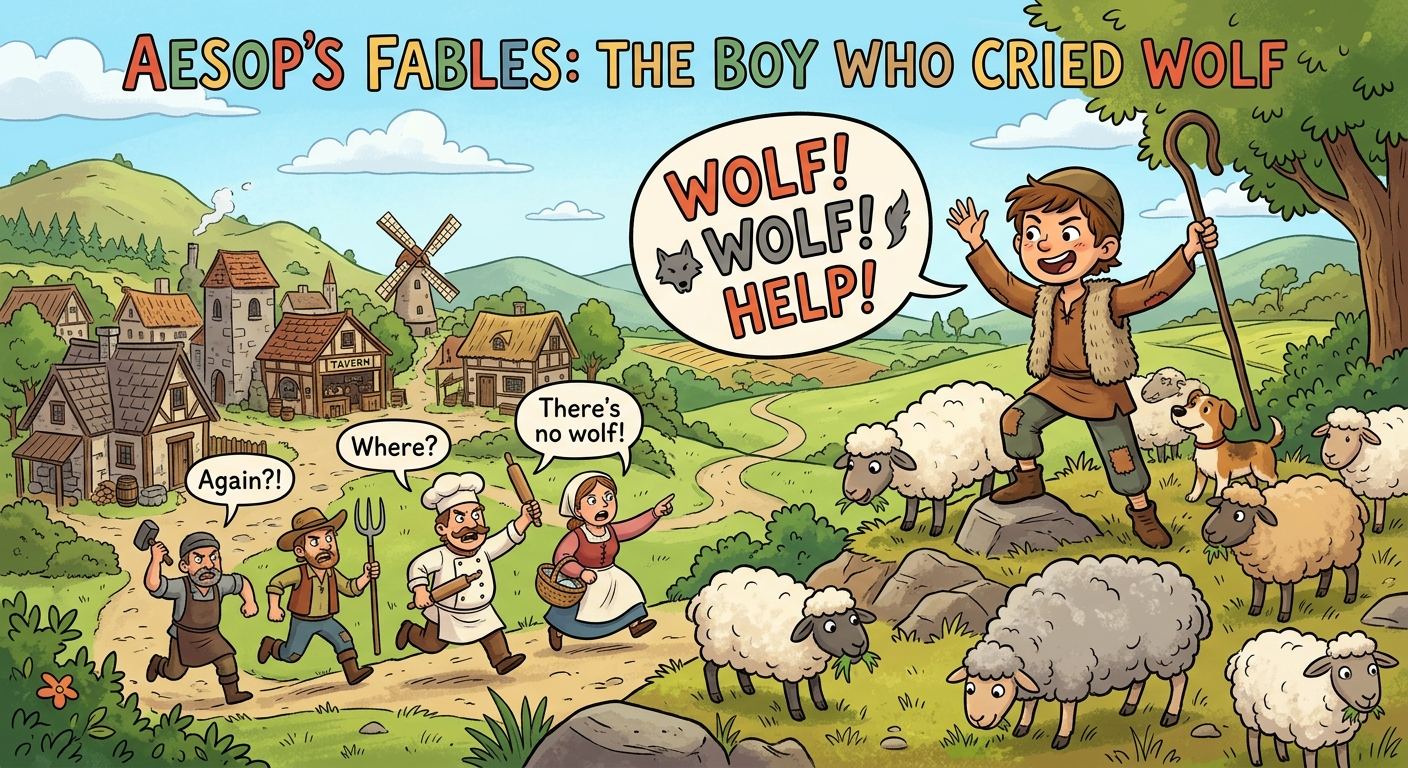
\includegraphics[width=\linewidth,keepaspectratio]{figures/aesop_wolf}
  \end{columns}
\end{frame}

\begin{frame}{Not all opinions are equal}
  \begin{columns}[T]
    \column{0.46\textwidth}
    \textbf{Majority voting}\\[0.5em]
    \small
    5 reviewers\\
    4 approve, 1 rejects\\
    $\downarrow$\\
    \textbf{APPROVE}\\[0.8em]
    \textit{What if the person\\shouting ``Wolf!''\\is usually right?}

    \column{0.46\textwidth}
    \pause
    \textbf{WaRF}\\[0.5em]
    \small
    \textcolor{auditor}{AUDITOR}\\
    \small\textit{historically reliable in this domain}\\[0.6em]
    \textcolor{testfoc}{TEST-FOCUSED}\\
    \small\textit{historically unreliable in this domain}\\[0.8em]
    \alert{Everyone gets a vote.}\\
    Not every vote gets\\
    the same weight.
  \end{columns}

  \vfill
  \small
  \textit{The agents reason about the code.\ \ WaRF reasons about the agents.}\\
  \scriptsize $\omega$ is not assigned — estimated from oracle-labelled history, separately per domain.
\end{frame}

\begin{frame}[standout]
  \Large Let's see what that\\actually looks like.
\end{frame}
\addtocounter{framenumber}{1}

\begin{frame}{What just happened?}
  \small
  \begin{tabular}{ll}
    \toprule
    Agent & Vote \\
    \midrule
    \textcolor{auditor}{AUDITOR}      & \textcolor{red}{REJECT} \\
    \textcolor{advocate}{ADVOCATE}    & \textcolor{red}{REJECT} \\
    \textcolor{boundary}{BOUNDARY}    & \textcolor{red}{REJECT}
                                        \quad \alert{$\leftarrow$ threshold crossed} \\
    \textcolor{skeptic}{SKEPTIC}      & \textit{skipped} \\
    \textcolor{testfoc}{TEST-FOCUSED} & \textit{skipped} \\
    \bottomrule
  \end{tabular}

  \vfill
  Each vote updates a running evidence score $\Lambda = \sum_i \omega_i \cdot \Delta_i$.\\
  WaRF stops when $\Lambda$ crosses a predefined boundary.\\[0.5em]
  \alert{WaRF does not count votes.}\\
  It accumulates evidence, weighted by each reviewer's track record,\\
  until a decision threshold is crossed.\\[0.4em]
  \scriptsize
  \href{run:../.warf/slide06.html}{The exact trace from this session is shown alongside.}
\end{frame}

\begin{frame}{Does WaRF know when it's right?}
  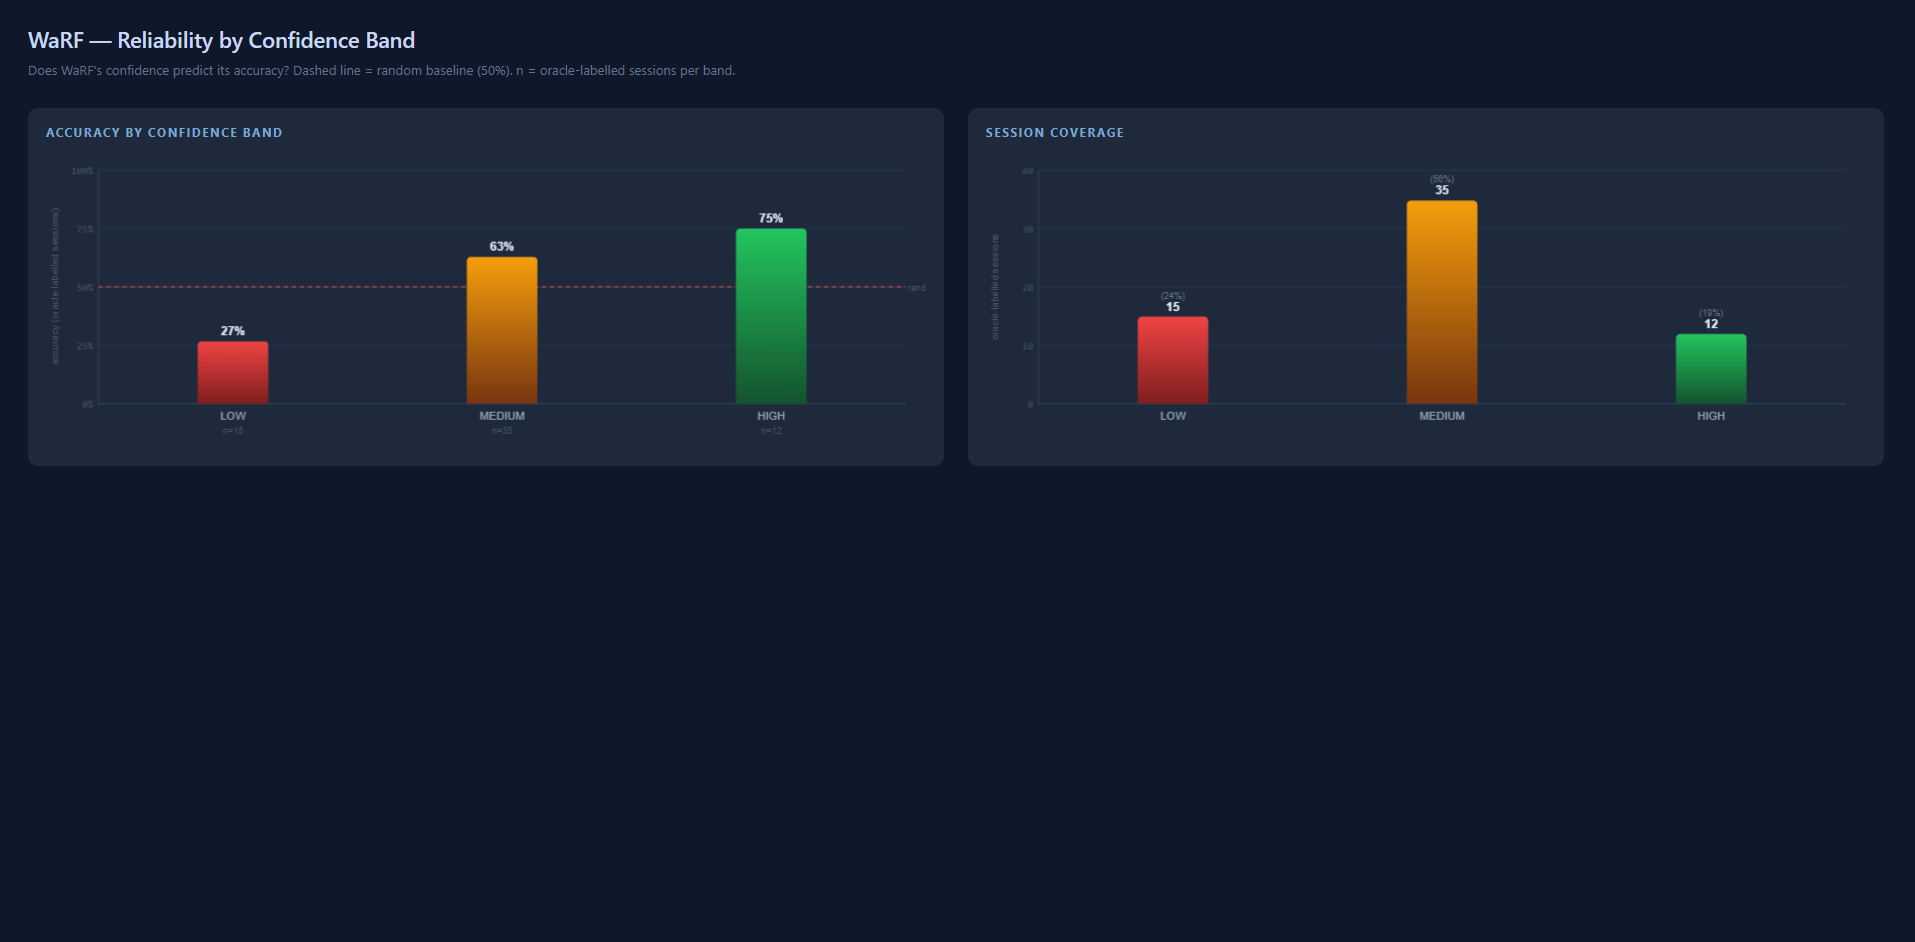
\includegraphics[width=\linewidth]{figures/reliability_diagram.png}

  \vfill
  \small
  In the calibration corpus, higher confidence coincides with higher accuracy.\\[0.3em]
  \textit{Preliminary: calibration and evaluation currently overlap.}\\[0.4em]
  \scriptsize
  \href{run:../.warf/confidence_calibration.html}{Exact rates and session counts $\rightarrow$}
\end{frame}

\begin{frame}{What early stopping buys}
  \footnotesize
  {\color{gray} FULL REVIEW — all 5 agents queried}\\[3pt]
  \textcolor{auditor}{\textbf{AUDITOR}} $\to$
  \textcolor{advocate}{\textbf{ADVOCATE}} $\to$
  \textcolor{boundary}{\textbf{BOUNDARY}} $\to$
  \textcolor{skeptic}{\textbf{SKEPTIC}} $\to$
  \textcolor{testfoc}{\textbf{TEST-FOCUSED}}\\[2pt]
  {\color{gray!35}\rule{\linewidth}{4pt}}
  \hspace{0.2em}\scriptsize\color{gray}$\leftarrow$ tokens spent\\[8pt]

  {\color{gray} EARLY STOP — SPRT boundary crossed at agent 3}\\[3pt]
  \textcolor{auditor}{\textbf{AUDITOR}} $\to$
  \textcolor{advocate}{\textbf{ADVOCATE}} $\to$
  \textcolor{boundary}{\textbf{BOUNDARY}} $\to$
  \alert{$\checkmark$\ \textbf{DECISION}}\\[2pt]
  {\color{gray!35}\rule{0.60\linewidth}{4pt}}
  \hspace{0.2em}\scriptsize\color{gray}$\leftarrow$ tokens spent\\

  \vfill
  \small
  Fewer agent calls are a consequence of sufficient evidence — not the optimisation target.\\[0.3em]
  \scriptsize
  \href{run:../.warf/token_cost_chart.html}{Observed token savings and stopping rates $\rightarrow$}
\end{frame}

\begin{frame}{It actually learns}
  
\begin{tikzpicture}
  \begin{axis}[
    width=0.90\textwidth, height=0.52\textheight,
    xlabel={\footnotesize oracle updates (SECURITY domain)},
    ylabel={\footnotesize $\hat\omega$},
    xlabel style={color=white!70!black},
    ylabel style={color=white!70!black, yshift=2pt},
    tick label style={font=\tiny, color=white!55!black},
    axis line style={color=gray!45},
    ymajorgrids=true,
    grid style={color=gray!18, line width=0.3pt},
    xmin=0, xmax=10, ymin=0.05, ymax=0.88,
    ytick={0.25, 0.5, 0.75},
    xtick=\empty,
    legend style={
      at={(1.02,1.01)}, anchor=north west,
      font=\tiny, fill=black!85, text=white!80!black,
      draw=gray!35, inner sep=3pt, row sep=-1pt,
    },
    legend cell align=left,
  ]
  \addplot[red!45, dashed, thin, forget plot]
    coordinates {(0,0.5)(10,0.5)};
  \addplot[color=auditor, line width=1.5pt, smooth]
    coordinates {(0,0.60)(2,0.72)(4,0.79)(5,0.65)(6,0.56)(7,0.60)(8,0.64)(9,0.68)(10,0.72)};
  \addlegendentry{good domain fit}
  \addplot[color=testfoc, line width=1.5pt, smooth]
    coordinates {(0,0.50)(1,0.42)(2,0.33)(3,0.25)(4,0.18)(5,0.27)(6,0.36)(7,0.43)(8,0.48)(9,0.51)(10,0.53)};
  \addlegendentry{poor domain fit}
  \addplot[gray!50, dashed, thin, forget plot]
    coordinates {(4.5,0.05)(4.5,0.88)};
  \node[font=\tiny, color=gray!60, rotate=90, anchor=south]
    at (axis cs:4.7,0.44) {labelling event};
  \end{axis}
  \end{tikzpicture}

  \vfill
  \small
  \textcolor{gray}{\textit{Case studies} (SECURITY domain):}\\[0.2em]
  AUDITOR \& ADVOCATE approved a urllib3 TLS change;\\
  upstream reverted it, oracle said REJECT --- their SECURITY weights drop.\\[0.3em]
  TEST-FOCUSED over-rejects mature library code.\\
  WaRF learns to trust it differently in that context.\\[0.3em]
  \alert{Weights are not measures of quality --- they are estimates of agent--domain fit.}\\[0.4em]
  \scriptsize
  \href{run:../.warf/weight_trajectories.html}{Live weight trajectories for all agents $\rightarrow$}
\end{frame}

\begin{frame}[standout]
  \Large One more.\\[0.5em]
  \normalsize This time the agents disagree.
\end{frame}
\addtocounter{framenumber}{1}

\begin{frame}{Can Debate Resolve Disagreement?}
  \small
  \begin{tabular}{p{2.8cm}p{1.8cm}p{4.2cm}}
    \toprule
    Case & Outcome & Why \\
    \midrule
    Authentication bug
      & \textcolor{green!60!black}{\textbf{Fixed}}
      & Correct minority had a verifiable argument \\[0.5em]
    False belief
      & \textcolor{gray}{\textbf{No change}}
      & Correct explanation did not penetrate \\[0.5em]
    Plausible misconception
      & \textcolor{red}{\textbf{Worse}}
      & Wrong argument persuaded the correct minority \\
    \bottomrule
  \end{tabular}

  \vfill
  \small
  Debate can improve a decision. It can also amplify an error.\\[0.5em]
  \begin{tabular}{ll}
    \textit{``Do you revise?''}      & $\to$ convergence pressure \\[0.2em]
    \textit{``Maintain or revise?''} & $\to$ minority keeps its footing \\
  \end{tabular}\\[0.3em]
  \small\textit{In our experiments, even prompt wording changed group behaviour.}\\[0.4em]
  \alert{Persuasion $\neq$ correctness.}
\end{frame}

\begin{frame}{When WaRF Fails}
  \small
  \begin{tabular}{p{2.8cm}p{6.4cm}}
    \toprule
    Failure mode & What happens \\
    \midrule
    \textbf{Persona bias}
      & Two personas share a framing blind spot ---\\
      & AUDITOR and ADVOCATE read intent, miss the omission \\[0.4em]
    \textbf{Knowledge gap}
      & Credential leak in \texttt{requests}:\\
      & nobody recognises the pattern --- even the one REJECT cites other reasons \\[0.4em]
    \textbf{False consensus}
      & Correct minority capitulates in debate ---\\
      & persuasive wrong argument wins \\
    \bottomrule
  \end{tabular}

  \vfill
  \small
  \alert{More agents of the same kind make knowledge-gap failures worse.}\\
  WaRF cannot manufacture knowledge that none of its agents possess.
\end{frame}

{
\setbeamercolor{background canvas}{bg=black}
\begin{frame}[plain]
  \vfill
  \centering
  \LARGE
  \textcolor{white}{Everyone gets a vote.}\\[0.8em]
  \textcolor{white}{Not every vote gets the same weight.}
  \vfill
\end{frame}
}

\begin{frame}{What's next}
  \begin{itemize}
    \item More history $\to$ better calibration $\to$ less manual labelling

    \item More domains, more agent personas
    \item Open: should the oracle reward \textit{reasoning quality},\\
          not just vote correctness?
  \end{itemize}

  \vfill
  \small
  \textit{Prior art:}
  \textsc{ConSol} (2025, arXiv 2503.17587) applies SPRT to a single model at varied temperature.
  A ConSol-style pool inside WaRF --- \textsc{Skeptic}$\times$5 --- rejected all 4 files it was given,
  each at \textsc{High} confidence, including clean code (\texttt{hooks.py}, \texttt{sessions.py}):
  five identical pessimistic personas cannot say \textsc{approve}.
  The mixed panel approved \texttt{hooks.py} because \textsc{Advocate} and \textsc{Auditor} pushed back.
  Rerun on a balanced 12-file set with today's personas: accuracy is a tie (mixed panel 11/12, five
  \textsc{Auditor}s 10/12, five \textsc{Skeptic}s 10/12) --- but only the clones were confidently wrong:
  five \textsc{Skeptic}s unanimously rejected clean code at \textsc{High} confidence.\\[0.2em]
  \textit{Temperature diversity gives you noise around one perspective.
  Persona diversity gives you genuinely different expertise.}
\end{frame}

\begin{frame}{Why not two well-calibrated agents?}
  \begin{columns}[T]
    \column{0.52\textwidth}
    \small
    For any pool of $n$ agents, the maximum signal
    that can accumulate in one direction is:
    \[|\Lambda|_{\max}(n) = \Bigl(\sum_{i=1}^{n}\omega_i\Bigr)\times LLR_{ABS}\]
    Early stopping requires $|\Lambda|_{\max}$ to reach
    a boundary: $|\lambda_B|\approx 2.25$ (REJECT) or $\lambda_A\approx 2.89$ (APPROVE).\\[0.5em]
    At current $\omega$ values, the best two agents
    fall \alert{below both boundaries} — no early stop, never \textsc{High}.\\[0.4em]
    Adding a third agent crosses the REJECT boundary.\\
    \href{run:../.warf/why_not_two_agents.html}{Current weights \& boundary chart $\rightarrow$}

    \column{0.44\textwidth}
    \vspace{0.5em}
    \small
    A fraction of 5-agent sessions fire early
    with \alert{High} confidence.\\[0.5em]
    \textit{Structurally impossible with $n=2$.}\\[0.5em]
    On those sessions:\\
    5 agents is \alert{cheaper} (3 used)\\
    and \alert{more confident}\\
    than 2 agents (never \textsc{High}).
  \end{columns}

  \vfill
  \scriptsize\textit{Counter to arXiv\,2604.02460:
  code review $\neq$ reasoning task.
  Ensemble value is in \textsc{High}-confidence early stops, not average accuracy.}
\end{frame}

\end{document}
